\documentclass[12 pt]{article}
\usepackage[utf8]{inputenc}
\usepackage{a4}
\usepackage{indentfirst}
\usepackage{graphicx}
\usepackage{float}
\usepackage{tabularx}
\usepackage{multicol}
\usepackage{tikz, adjustbox}
\usepackage[most]{tcolorbox}
\usepackage{wrapfig}
\usepackage{amssymb}
\usepackage{amsmath}
\usepackage{hyperref}
\newcolumntype{M}[1]{>{\centering\arraybackslash}m{#1}}
\usepackage{titlesec}
\usepackage{listings}
\usepackage{esint}
\usepackage{xcolor}
\definecolor{codegreen}{rgb}{0,0.6,0}
\definecolor{codegray}{rgb}{0.5,0.5,0.5}
\definecolor{codepurple}{rgb}{0.58,0,0.82}
\definecolor{backcolour}{rgb}{0.95,0.95,0.92}
\emergencystretch=1em
\lstdefinestyle{mystyle}{
    backgroundcolor=\color{backcolour},  
    commentstyle=\color{codegreen},
    keywordstyle=\color{magenta},
    numberstyle=\tiny\color{codegray},
    stringstyle=\color{codepurple},
    basicstyle=\footnotesize\ttfamily,
    breakatwhitespace=false,         
    breaklines=true,                 
    captionpos=b,                    
    keepspaces=true,                 
    numbers=left,                    
    numbersep=5pt,                  
    showspaces=false,                
    showstringspaces=false,
    showtabs=false,                  
    tabsize=2,
    frame=single,
}
\lstset{style=mystyle}
% Yellow:
\definecolor{BgYellow}{HTML}{FFF59C}
\definecolor{FrameYellow}{HTML}{F7A600}
% Pink:
\definecolor{BgPink}{HTML}{EF6FA7}
\definecolor{FramePink}{HTML}{E5446E}


% Yellow Sticky Note (YStkyNote):
\newtcolorbox{YStkyNote}[1][]{%
    enhanced,
    before skip=2mm,after skip=2mm, 
    width=0.6\textwidth, % width of the sticky note
    boxrule=0.2mm,
    colback=BgYellow, colframe=FrameYellow, % Colors
    attach boxed title to top left={xshift=0cm,yshift*=0mm-\tcboxedtitleheight},
    varwidth boxed title*=-3cm,
    % The titlebox:
    boxed title style={frame code={%
        \path[left color=FrameYellow,right color=FrameYellow,
        middle color=FrameYellow]
        ([xshift=-0mm]frame.north west) -- ([xshift=0mm]frame.north east)
        [rounded corners=0mm]-- ([xshift=0mm,yshift=0mm]frame.north east)
        -- (frame.south east) -- (frame.south west)
        -- ([xshift=0mm,yshift=0mm]frame.north west)
        [sharp corners]-- cycle;
        },interior engine=empty,
    },
    sharp corners,rounded corners=southeast,arc is angular,arc=3mm,
    % The "folded paper" in the bottom right corner:
    underlay={%
        \path[fill=BgYellow!80!black] ([yshift=3mm]interior.south east)--++(-0.4,-0.1)--++(0.1,-0.2);
        \path[draw=FrameYellow,shorten <=-0.05mm,shorten >=-0.05mm,color=FrameYellow] ([yshift=3mm]interior.south east)--++(-0.4,-0.1)--++(0.1,-0.2);
        },
    drop fuzzy shadow, % Shadow
    fonttitle=\bfseries, 
    title={#1}
}
% Pink Sticky Note (PStkyNote):
\newtcolorbox{PStkyNote}[1][]{%
    enhanced,
    before skip=2mm,after skip=2mm, 
    width=0.4\textwidth, % width of the sticky note
    boxrule=0.2mm, 
    colback=BgPink, colframe=FramePink, % Colors
    attach boxed title to top left={xshift=0cm,yshift*=0mm-\tcboxedtitleheight},
    varwidth boxed title*=-3cm,
    % The titlebox:
    boxed title style={frame code={%
        \path[left color=FramePink,right color=FramePink,
        middle color=FramePink]
        ([xshift=-0mm]frame.north west) -- ([xshift=0mm]frame.north east)
        [rounded corners=0mm]-- ([xshift=0mm,yshift=0mm]frame.north east)
        -- (frame.south east) -- (frame.south west)
        -- ([xshift=0mm,yshift=0mm]frame.north west)
        [sharp corners]-- cycle;
        },interior engine=empty,
    },
    sharp corners,rounded corners=southeast,arc is angular,arc=3mm,
    % The "folded paper" in the bottom right corner:
    underlay={%
        \path[fill=BgPink!80!black] ([yshift=3mm]interior.south east)--++(-0.4,-0.1)--++(0.1,-0.2);
        \path[draw=FramePink,shorten <=-0.05mm,shorten >=-0.05mm,color=FramePink] ([yshift=3mm]interior.south east)--++(-0.4,-0.1)--++(0.1,-0.2);
        },
    drop fuzzy shadow, % Shadow
    fonttitle=\bfseries, 
    title={#1}
}
\title{\huge{Lecture Notes 1: Vector Operators}}
\author{}
\date{}
\begin{document}
\maketitle
\tableofcontents
\newpage

\section{Introduction}
\textbf{A vector operator: }\begin{itemize}
    \item A differential operator in vector calculus
    \item It can be used to move from the integral form of the equation to its differential one.
    \item The most important operators:\begin{itemize}
        \item Gradient
        \item Divergence 
        \item Curl
    \end{itemize}
\end{itemize}
\section{Gradient}
It's a vector that represents the direction and the magnitude of the maximum space rate of increase of a scalar function.
$$
\nabla V=\frac{\partial{v}}{\partial{x}} \underline{u_x} +\frac{\partial{v}}{\partial{y}} \underline{u_y}+\frac{\partial{v}}{\partial{z}} \underline{u_z}
$$
\subsection{Visualization}
    \begin{figure}[H]
    \centering
    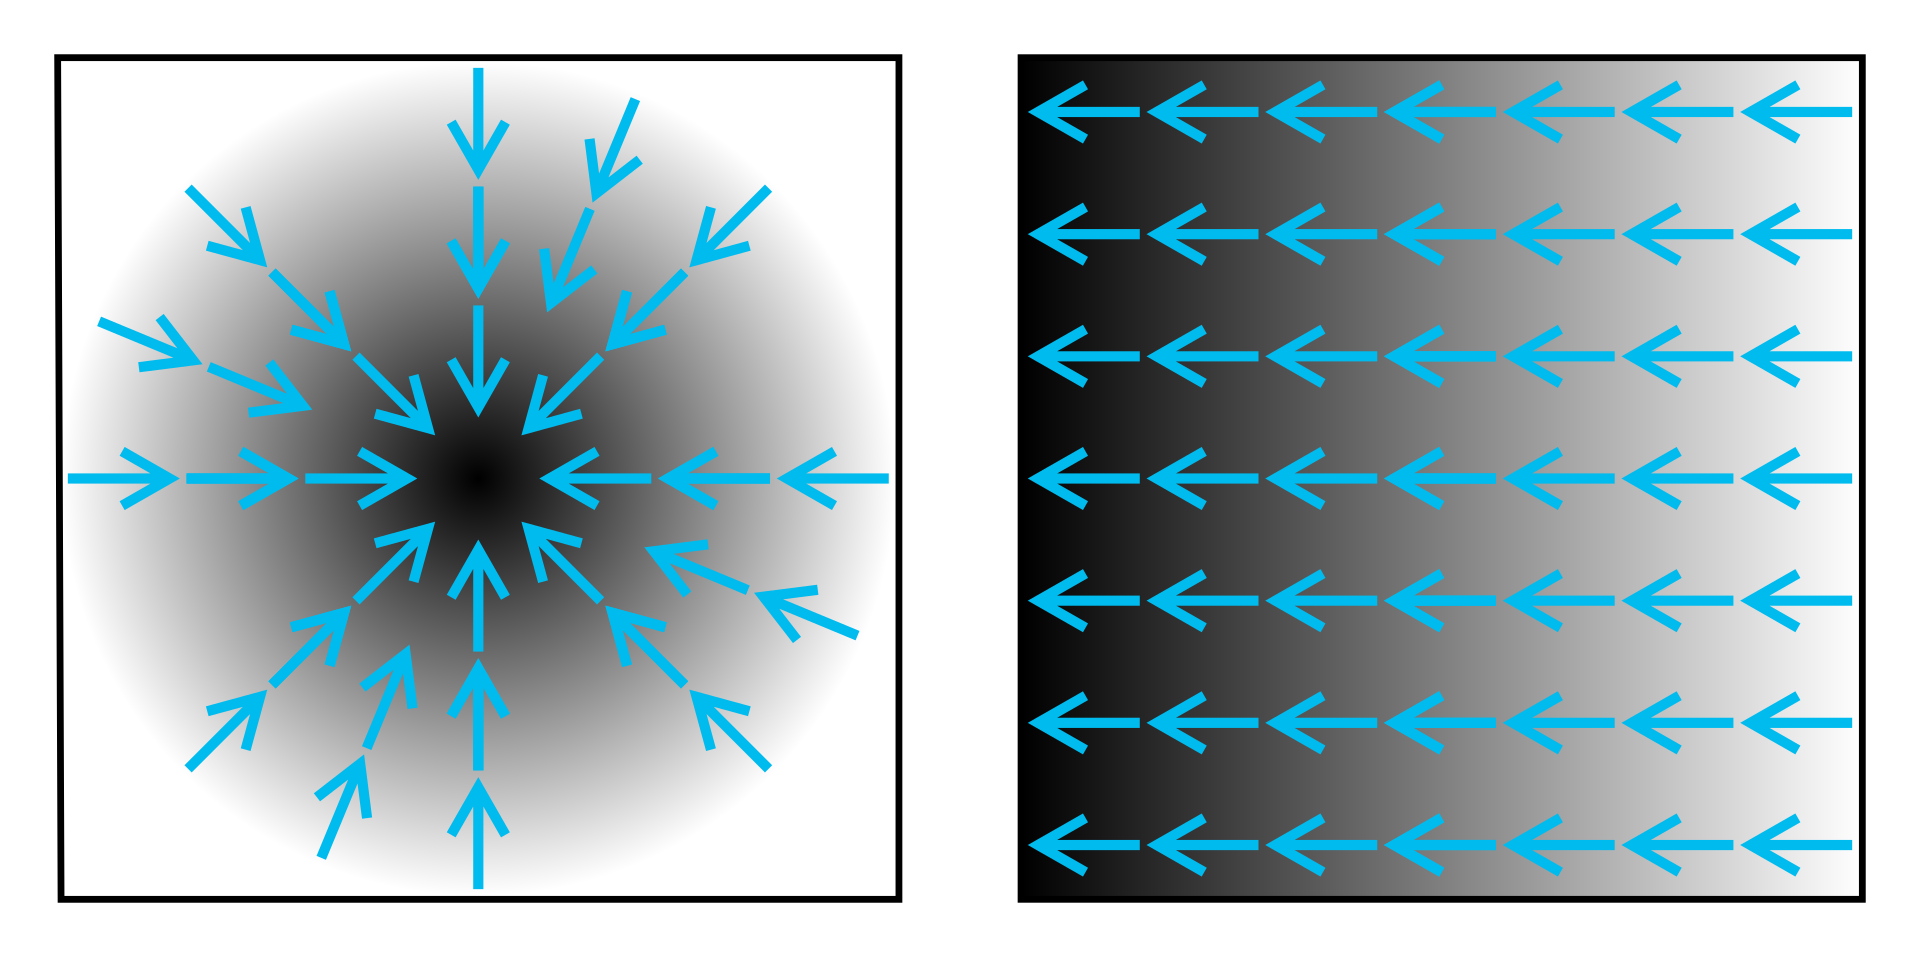
\includegraphics[scale=0.15]{./images/gradient}
    \label{gradient} 
\end{figure}
The gradient, represented by the blue arrows, denotes the direction of the greatest change of a scalar function. The values of the function are represented in greyscale and increase in value from white (low) to dark (high).
\section{Divergence}
The divergence represents the volume density of the outward flux of a vector field from an infinitesimal volume around a given point. 
$$
\nabla\cdot\underline{A}=\lim_{\Delta v \to 0} \frac{\oint_{s}\underline{A}\cdot ds}{\Delta v}=\frac{\partial{A_x}}{\partial{x}}+\frac{\partial{A_y}}{\partial{y}}+\frac{\partial{A_z}}{\partial{z}}
$$
\subsection{Physical meaning}
Divergence produces a scalar quantity which can be:
\begin{itemize}
    \item \textbf{+ve}: This means that the point acts as a source of flux,(e.g: +ve charge)
    \item \textbf{-ve}: This means that the point acts as a sink of flux, (e.g: -ve charge)
    \item \textbf{zero}: This means that the point is:\begin{itemize}
        \item source free (or number of source = number of sink)
        \item $\underline{A}$ is called solenoidal field (e.g: Magnetic field)
    \end{itemize}
\end{itemize}
\subsection{Visualization}
    \begin{figure}[H]
    \centering
    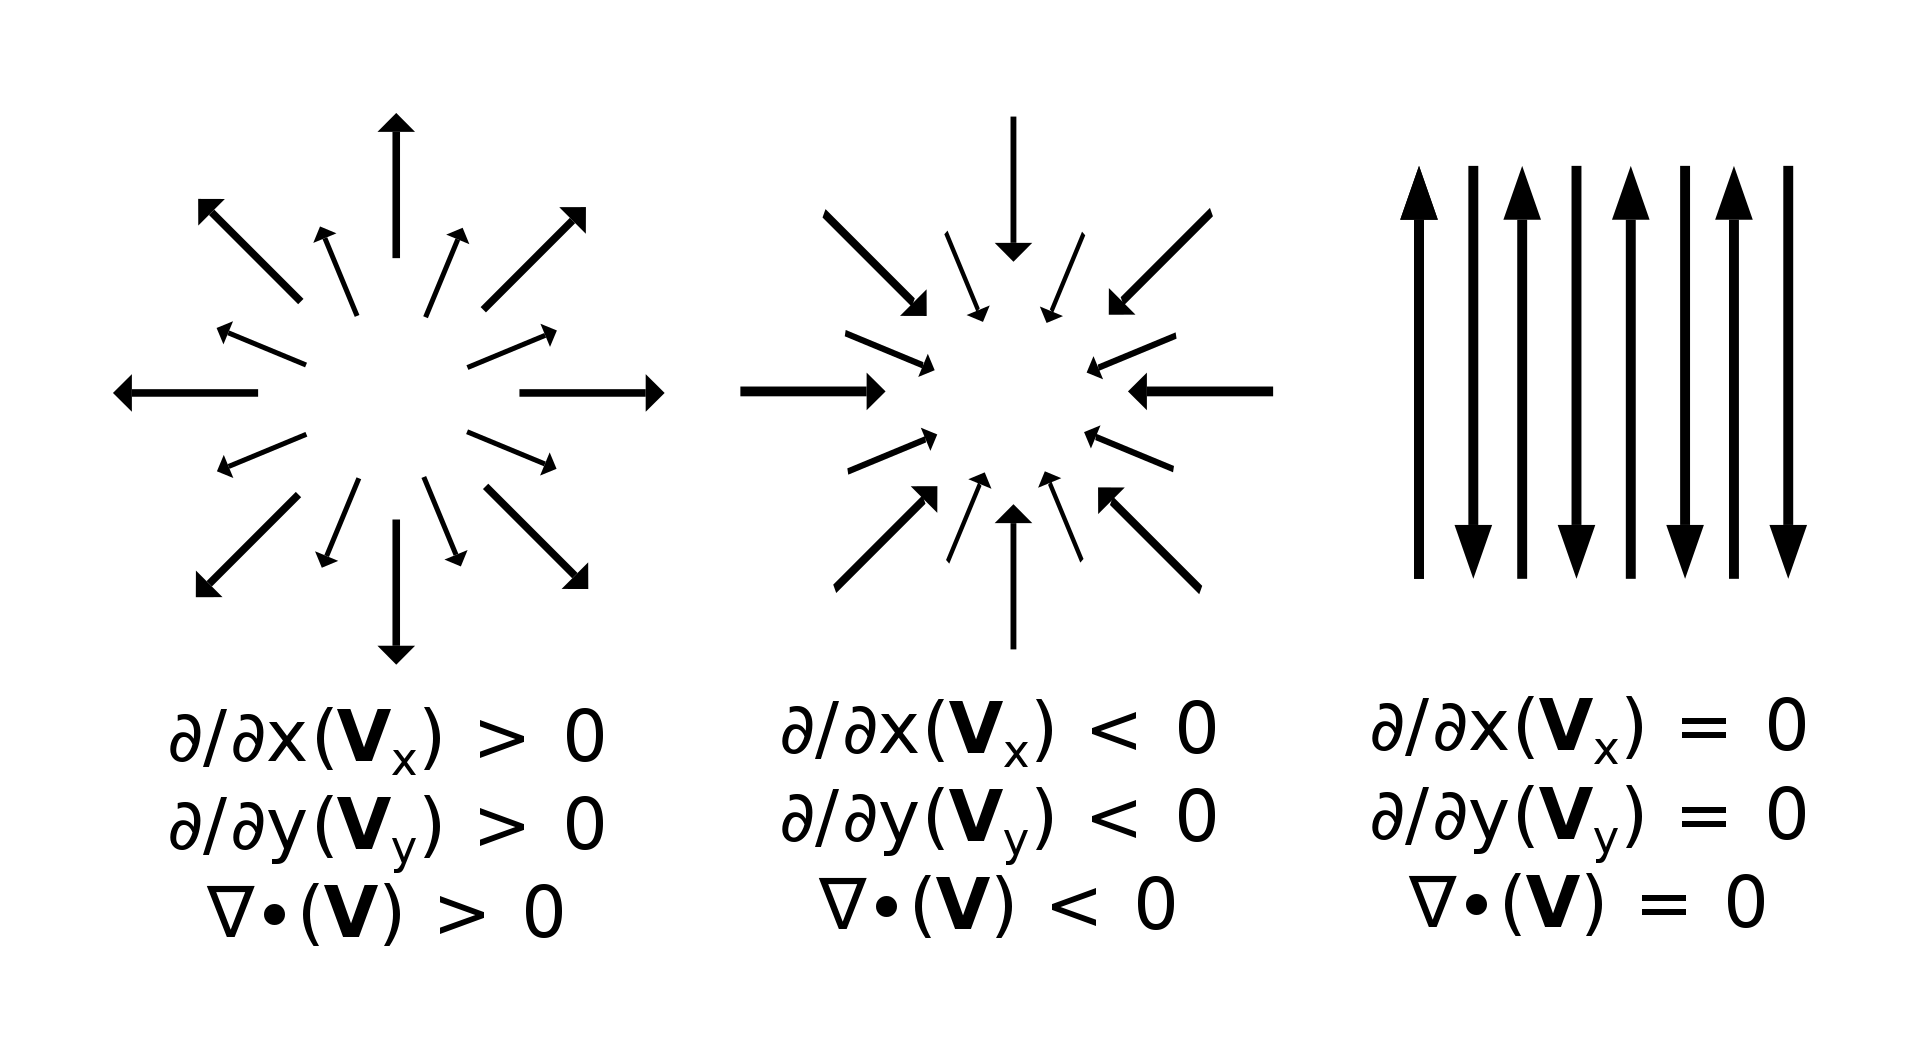
\includegraphics[scale=0.15]{./images/divergence}
    \label{divergence} 
\end{figure}
\newpage
\section{Curl}
\textbf{Circulation:} It is the amount of force(vortex source) that pushes along a closed boundary or path, such as a circle.

\textbf{Curl:} It's simply the circulation per unit Area when the area tends to zero, and its direction is the normal to the area
$$
\nabla\times\underline{A}=\lim_{\Delta s \to 0} \frac{ \underline{u_n}\oint_{c}\underline{A}\cdot dl}{\Delta s}
$$
$$
\nabla \times \underline{A}=
\begin{vmatrix}
u_x  & u_y  & u_z  \\ 
\frac{\partial{}}{\partial{x}} & \frac{\partial{}}{\partial{y}} & \frac{\partial{}}{\partial{z}} \\ 
A_x & A_y & A_z 
\end{vmatrix}
$$
\subsection{Physical meaning}
The magnitude of the curl vector at a point measures how quickly the surrounding particles rotate around this point, or in other words, the curl at a point is a measure of the vector field ’s “spin” at that point. and its direction follows the right hand rule (check visualization below):
\begin{itemize}
    \item \textbf{+ve:} the pushing force (vortex source) is along $u_n$
    \item \textbf{-ve:} the pushing force (vortex source) is opposite to $u_n$
    \item \textbf{zero: } \begin{itemize}
        \item no pushing force (vortex source) is crossing $\Delta s$ 
        \item $\underline{A}$ is called irrotational field (e.g: Electrostatic field)
    \end{itemize}
\end{itemize}
\subsection{Visualization}
    \begin{figure}[H]
    \centering
    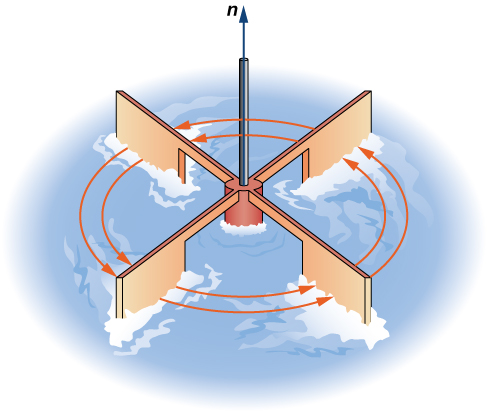
\includegraphics[scale=0.75]{./images/curl}
    \label{curl} 
\end{figure}
\end{document}
